%%%%%%%%%%%%%%%%%%%%%%preface.tex%%%%%%%%%%%%%%%%%%%%%%%%%%%%%%%%%%%%%%%%%
% sample preface
%
% Use this file as a template for your own input.
%
%%%%%%%%%%%%%%%%%%%%%%%% Springer %%%%%%%%%%%%%%%%%%%%%%%%%%

\preface

%% Please write your preface here
% Use the template \emph{preface.tex} together with the Springer document class SVMono (monograph-type books) or SVMult (edited books) to style your preface in the Springer layout.

% A preface\index{preface} is a book's preliminary statement, usually written by the \textit{author or editor} of a work, which states its origin, scope, purpose, plan, and intended audience, and which sometimes includes afterthoughts and acknowledgments of assistance. 

% When written by a person other than the author, it is called a foreword. The preface or foreword is distinct from the introduction, which deals with the subject of the work.

% Customarily \textit{acknowledgments} are included as last part of the preface.

\paragraph{Origin}

This book describes the \Digraph collection of Python3 resources for implementing decision aid algorithms in the context of a bipolar-valued outranking approach. These computing resources are useful in the field of Algorithmic Decision Theory and more specifically in outranking based Multiple Criteria Decision Aid (MCDA). They provided practical tools for a Master Course on Algorithmic Decision Theory taught at the University of Luxembourg. Their development, starting in 2010 covers a period of more than ten years, was stepwise and the reader might find some cases of backward compatibility problems.

\paragraph{Scope}

The \Digraph documentation, available \href{https://digraph3.readthedocs.io/en/latest/}{on the Read The Docs site}, describes the Python3 resources for implementing decision aid algorithms in the context of a bipolar-valued outranking approach. These computing resources are useful in the field of Algorithmic Decision Theory and more specifically in outranking based Multiple Criteria Decision Aid (MCDA). They provide practical tools for a Master Course on Algorithmic Decision Theory taught at the University of Luxembourg.

\paragraph{Plan}

\noindent The book contains, first, a set of chapters introducing the \Digraph resources and the main formal objects discussed in this book, like digraphs and outranking digraphs. A second part presents evaluation models, essentially performance tableaux, and decision methods and tools. Some chapters are problem oriented and show how to compute the winner of an election, how to build a best choice recommendation, or how to linearly rank or rate with multiple incommensurable performance criteria.A third part present a case study for best choice, for a ranking and for a rating decision problem. A fourth Section presents more advanced topics showing some pearls of bipolar-valued epistemic logic. A last part concerns simple undirected graphs and present operational aspects of computing maximal independent sets (MISs) and kernels in graphs and digraphs. The tutorial about split, interval and permutation graphs is inspired by Martin Golumbic ‘s book on Algorithmic Graph Theory and Perfect Graphs. We also provide a tutorial on tree graphs and spanning forests.

\paragraph{Intended audience}

Master students and doctoral candidates in Computer Science, Engineering Sciencess and Computational Management Sciences taking a course on Algorithmic Decision Theory, Multiple criteria Decision Aid or DEcision Analysis.

\paragraph{Aknowledgments}

This book contains many ideas, methods and tools that are not only the author’s. They have been borrowed from friends and colleagues: 

\vspace{0.5cm}
\begin{minipage}{7cm}
\emph{Denis Bouyssou, Luis Dias,}\\ 
\emph{Claude Lamboray, Patrick Meyer,}\\
\emph{Vincent Mousseau, Alex Olteanu,}\\
\emph{Marc Pirlot, late Bernard Roy,}\\
\emph{Alexis Tsouki\`as, Thomas Veneziano,}\\
and especially,\\
\emph{late Marc Roubens}.
\end{minipage}\quad
\begin{minipage}{3cm}
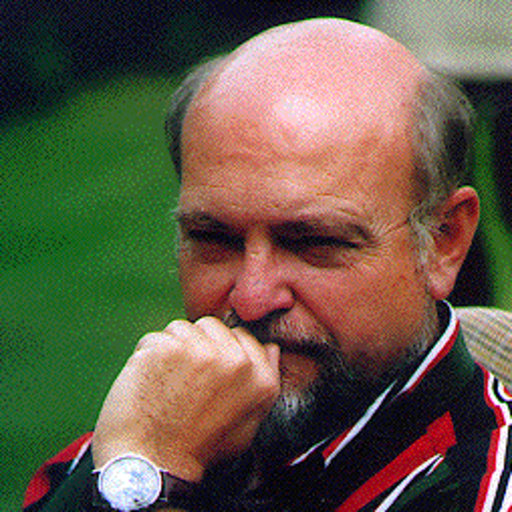
\includegraphics[width=3cm]{Figures/Marc-Roubens.jpg} \\
{\tiny \emph{Marc Roubens}}
\end{minipage}

\vspace{0.3cm}
Their help is gratefully acknowledged.

\vspace{\baselineskip}
\begin{flushright}\noindent
Luxembourg, 2021\hfill {\it Raymond Bisdorff}\\
%month year\hfill {\it Firstname  Surname}\\
\end{flushright}


